

\section{Funktion eines HF-Verstärkers}
Ein Verstärker ist ein elektronisches Gerät mit mindestens einem 
aktiven Bauelement, wie zum Beispiel einem Transistor.
Das Ziel eines Verstärkers ist es, das Ausgangssignal 
größer als das Eingangssignal zu machen. Da hierbei dem Signal Leistung hinzugefügt
wird, muss ein Verstärker eine eigene Energiequelle besitzen.
\\
Besonders in der Hochfrequenztechnik (HF) spielt der Verstärker eine wichtige
Rolle. Soll zum Beispiel mithilfe einer Antenne noch in weiter Entfernung ein Signal
gemessen werden, muss dieses zuerst verstärkt werden.
\\
Normalerweise werden im Hochfrequenzbereich Frequenzen von 10 kHz bis 100.000 MHz
verstärkt.
\clearpage
\section{Arbeitspunkteinstellung}
Der Arbeitspunkt einer elektronischen Schaltung beschreibt den 
Ruhezustand, wenn kein Signal angelegt ist.
Er liegt auf einem bestimmten Punkt der Kennlinie.
Je nach Einstellung kann die Schaltung unterschiedlich auf das Eingangssignal
reagieren.
\\
\\
\begin{figure}[h]
    \centering
    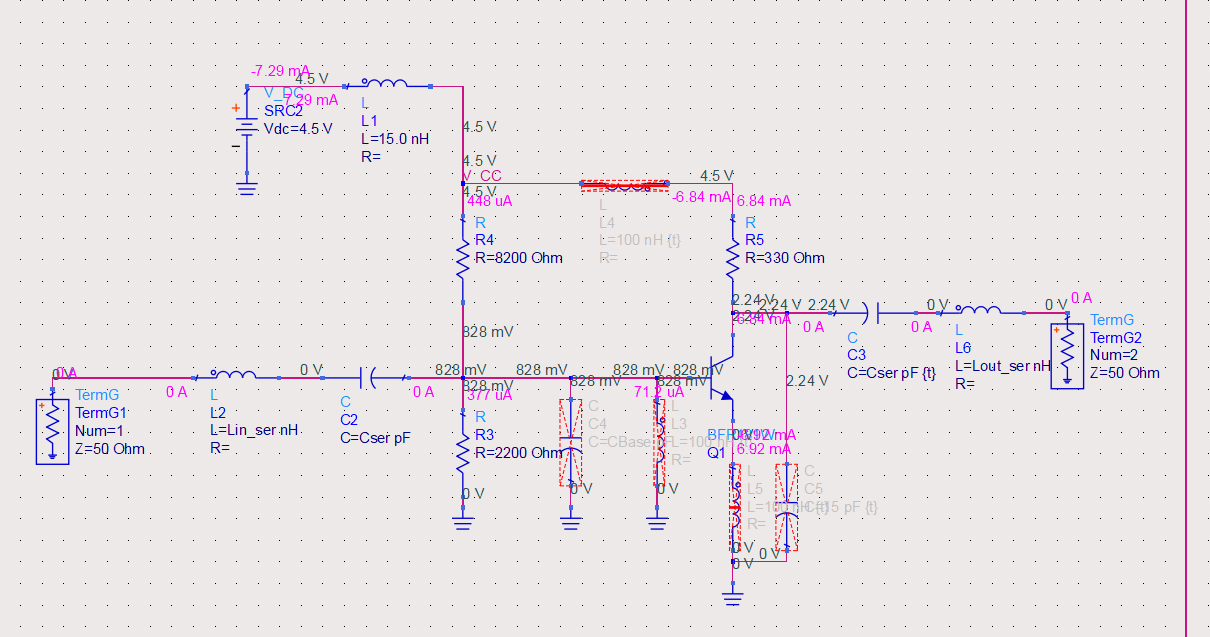
\includegraphics[width=1.0\textwidth]{Pictures/Schaltplan.png}
    \caption{Emitterschaltung}
\end{figure}
\\
\subsection{Dimensionierung des Kollektorwiderstandes}

 Folgende Spannungswerte seien gegeben:
 \begin{itemize}
     \item $U_{CC} = 4.8\,\mathrm{V}$
     \item $U_{BE} = 0.77\,\mathrm{V}$
 \end{itemize}

 Der Kollektorstrom $I_C$ wird auf $75\,\%$ des maximalen zulässigen Kollektorstroms \\$I_{C,\mathrm{max}} =20mA$  gesetzt. 
 Der Widerstandswert $R_5$ wird mit folgender Formel berechnet:
 \begin{equation}
     R_5 = \frac{U_{CC} - U_{CE}}{I_C} = \frac{4.8\,\mathrm{V}}{15\,\mathrm{mA}} = 320\,\Omega
 \end{equation}

 Bei der Verwendung der E12-Reihe wird eine Faustregel angewendet, nach der man die Widerstandswerte auf die nächstgelegene E12-Reihe aufrundet. 
 Somit beträgt der errechnete Widerstandswert von $R_5$ 330\,\(\Omega\). Dadurch wird der in den Kollektor eingehende Strom begrenzt, was eine Überlastung des Transistors im Dauerbetrieb verhindert. 
 Bei der Wahl eines niedrigeren Widerstandswertes würde der Kollektorstrom $I_C$ den maximalen Kollektorstrom $I_{C,\mathrm{max}}$ überschreiten, was zu einer Überlastung des Transistors führen würde.

\subsection{Dimensionierung des Basis-Spannungsteilers}
Der Basisstrom berechnet sich zu:
 \begin{equation}
     I_B = \frac{I_C}{\beta}
 \end{equation}
 Für einen typischen Verstärkungsfaktor $\beta = 100$ ergibt sich:
 \begin{equation}
     I_B = \frac{10\,\mathrm{mA}}{100} = 0{,}1\,\mathrm{mA} = 100\,\mu\mathrm{A}
 \end{equation}

 Der Querstrom des Spannungsteilers $I_Q$ sollte mindestens das 10-fache des Basisstroms betragen:
 \begin{equation}
     I_Q = 10 \cdot I_B = 1{,}0\,\mathrm{mA}
 \end{equation}

 Die Basisspannung $U_B$ ergibt sich zu:
 \begin{equation}
     U_B = U_{BE} + U_E \approx 0{,}77\,\mathrm{V}
 \end{equation}

 Angenommen, die Betriebsspannung ist $U_{CC} = 4{,}8\,\mathrm{V}$, ergeben sich für die Widerstände $R_4$ (oben) und $R_3$ (unten):
 \begin{align}
     R_3 &= \frac{U_B}{I_Q} = \frac{0{,}77\,\mathrm{V}}{1{,}0\,\mathrm{mA}} = 0{,}77\,\mathrm{k}\Omega \\
     R_4 &= \frac{U_{CC} - U_B}{I_Q} = \frac{4{,}8\,\mathrm{V} - 0{,}77\,\mathrm{V}}{1{,}0\,\mathrm{mA}} = 4{,}03\,\mathrm{k}\Omega
 \end{align}

 Nach der Berechnung ergibt sich für $R_3$ ein Wert von $0{,}77\,\mathrm{k}\Omega$. In der praktischen Simulation mit ADS zeigte sich jedoch, dass mit diesem Wert ein negatives Gain bei der S-Parameter-Simulation auftritt. Daher wird $R_3$ nach der E12-Reihe auf $1{,}0\,\mathrm{k}\Omega$ erhöht, um einen stabilen Arbeitspunkt und ein positives Verstärkungsverhalten zu gewährleisten.

 Mit der E12-Reihe werden gewählt:
 \begin{align*}
     R_3 &= 1{,}0\,\mathrm{k}\Omega \\
     R_4 &= 4{,}7\,\mathrm{k}\Omega
 \end{align*}

 Damit ist der Spannungsteiler dimensioniert, sodass im Arbeitspunkt ein Kollektorstrom von ca. $10\,\mathrm{mA}$ zu erwarten ist und die Simulation ein positives Gain liefert.

\section{Bedeutung der S-Parameter}
S-Parameter bzw. Streuparameter werden genutzt, um die HF-Eigenschaften eines
Netzwerks darzustellen. Sie werden benötigt, um zu verstehen, welche Anteile eines Signals
reflektiert, durchgelassen oder zwischen den Toren eines Netzwerks übertragen werden.
Sie werden komplex dargestellt, also mit Betrags- und Phasenkomponente.
\\
Die Indexnummerierung folgt dem Energiefluss.
\clearpage

\begin{itemize}
    \item Verläuft die Energie von Tor 1 in Tor 1, heißt der S-Parameter S11.
    \item Verläuft die Energie von Tor 2 in Tor 1, heißt der S-Parameter S21.
\end{itemize}
Somit können an einem Zweitor folgende S-Parameter auftreten:
\begin{itemize}
    \item S11 ist der Eingangsreflexionsfaktor. Dieser Parameter gibt an, wie viel des Eingangssignals zurückreflektiert wird.
    \item S21 ist der Vorwärtstransmissionsfaktor. Dieser Parameter gibt die Effizienz der Signalübertragung vom Eingang zum Ausgang an.
    \item S12 ist der Rückwärtstransmissionsfaktor. Dieser Parameter gibt an, wie gut Tor 1 von Signalen von Tor 2 isoliert ist.
    \item S22 ist der Ausgangsreflexionsfaktor. Dieser Parameter gibt an, wie viel des Ausgangssignals zurückreflektiert wird.
\end{itemize}
\subsection{Smith-Diagramm}
Das Smith-Diagramm ermöglicht die grafische Darstellung der S-Parameter.
Dafür werden der Real- und Imaginärteil des Reflexionsfaktors in Abhängigkeit von der Frequenz
aufgetragen und ermöglichen dadurch eine einfachere Impedanzanpassung.
\begin{figure}[h]
    \centering
    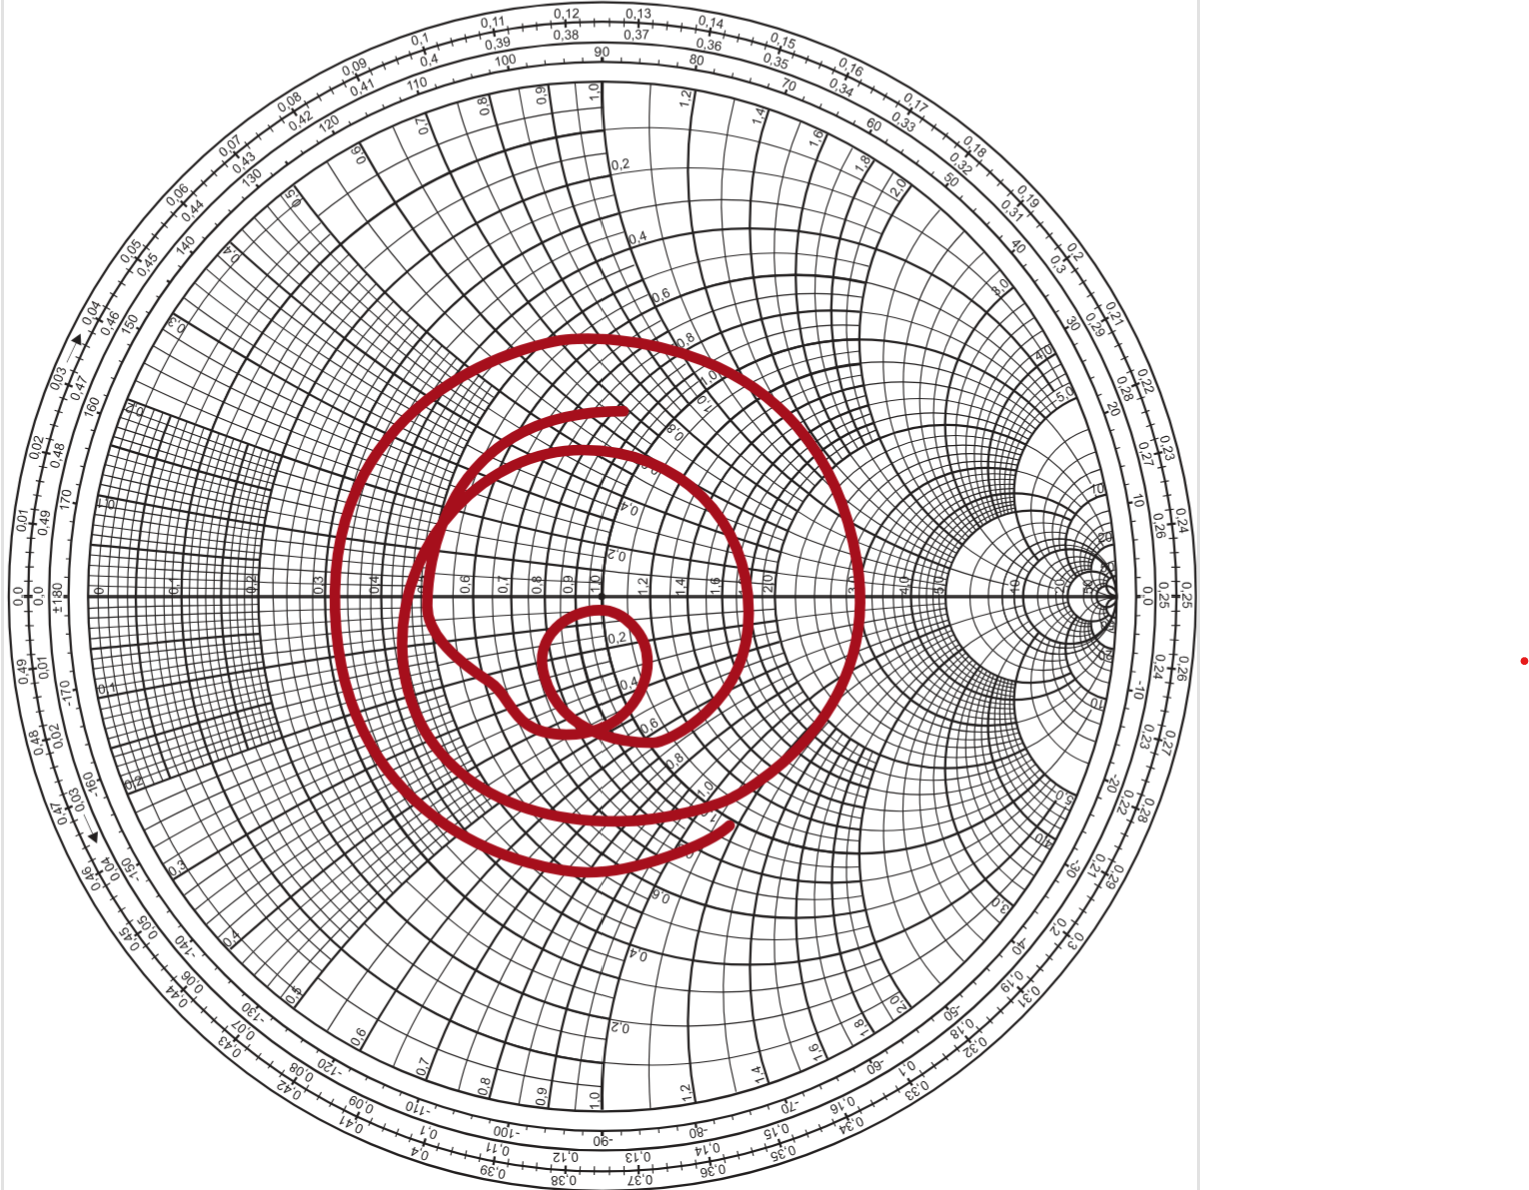
\includegraphics[width=0.4\textwidth]{Pictures/SmithDiagram.png}
    \caption{Smith-Diagramm Beispiel}
    \footnotesize{Quelle \url{https://www.rohde-schwarz.com/de/produkte/messtechnik/essentials-test-equipment/spectrum-analyzers/s-parameter-verstehen_257831.html#gallery-13}}
\end{figure}
\section{Koppelkondensator}
Die seriellen Kapazitäten bzw. Koppelkondensatoren in einer Emitterschaltung haben mehrere Aufgaben. Zum einen kompensieren sie Störungen, filtern den Gleichanteil
heraus und dienen gleichzeitig als Hochpass.
\clearpage
